\documentclass[12pt]{article}

% packages
\usepackage{setspace}
\usepackage{hyperref}
\usepackage{array}
\usepackage[margin=0.75in]{geometry}
\usepackage{amsmath,bm}
\usepackage{amssymb}
\usepackage{bbold}
\usepackage{physics}
\usepackage{xcolor}
\usepackage{indentfirst}
\usepackage{enumerate}
\usepackage{mathtools}
\usepackage{fancyhdr}

\pagestyle{fancy}
\fancyhf{}
\rhead{Creative Destruction Lab}
\lhead{Introductions to Projects}
\rfoot{Page \thepage}

\allowdisplaybreaks

\title{Project 3: Calculating Franck-Condon Factors}

\begin{document}

\maketitle

\thispagestyle{empty}

\subsection*{Motivation}

Spectroscopy is the study of how light and matter (atoms and molecules) interact.
Light can be absorbed by matter (\textit{absorption}) or matter can emit light (\textit{emission}).
It turns out that spectroscopy is scientists' main tool for discovering properties of molecules (e.g. their molecular structure, bond strengths, etc.) and for chemical identification. Picture for instance an astronomer taking spectroscopic measurements from a gas cloud located millions of light years away from the Earth. To determine what chemicals this gas cloud comprises of, they certainly cannot travel there and take a physical sample of the gas cloud. The astronomer is tasked with utilizing spectroscopic theory (i.e. models wherein numerical studies can be carried out efficiently) to explain what they see.

Countless other applications like drug discovery, magnetic-resonance imaging (MRI) and climate science rely heavily on spectroscopic methods and theory. This week, you'll familiarize yourself with calculating Franck Condon Factors (FCFs), which are useful in studying {\it vibronic} transitions in molecules. You'll also get to compare your calculations to real experiments.

\subsection*{Gaussian Boson Sampling}
As you have learned in Week 2 in the presentation by Xanadu, Boson Sampling is a powerful tool which demonstrates that a non-universal quantum computer can display exponential speedup over classical computers, especially in the quantum optics or photonics field\cite{huh2015boson,aaronson2011computational, harrow2017quantum, quesadaFranckCondonFactorsCounting2019}. For our purpose, Gaussian Boson Sampling (GBS), which uses Gaussian input states, can be used to calculate Franck-Condon Factors and can be used to generate vibronic spectra.

Franck-Condon Factors involve the overlap of the ``starting" and ``ending" wavefunctions of a transition and they are proportional to the amplitude of the vibronic spectrum. The method to calculate the Franck-Condon Factor between state $|m\rangle$ and $|n\rangle$ requires the use of the Doktorov operator, $U_{Dok}$, which allows the final state to be represented in terms of the initial state. The overlap can then be calculated as 

\begin{equation}
FCF=|\langle m|U_{Dok}|n\rangle|^2    ~.
\end{equation}

This Doktorov operator can be written in terms of displacement, $D_\alpha$, squeezing,$\Sigma_r$ and interferometer operators $U_1$, $U_2$ as\cite{killoran2019strawberry, bromley2020applications}:

\begin{equation}
U_{Dok}=D_\alpha U_2 \Sigma_r U_1    ~.
\end{equation}

A GBS device can be programmed to perform these operations for a particular molecule, therefore can be used to calculate the FCFs and, in turn, the vibronic spectrum of a molecule. You will have an opportunity to simulate this ``experiment'' in Task 3. 
\newpage

\subsection*{Your Tasks}

\subsubsection*{Task \#1}

In this task, you will calculate Franck-Condon Factors for H$_2-$H$_2^+$ using the harmonic oscillator approximation and compare to a real experiment! In a real experiment, we can excite many different vibronic transitions. We would therefore be able to calculate many FCFs that describe different vibronic transitions. For example, it could be that we see excitations corresponding to an H$_2$ molecule in its $n = 0$ vibrational state to H$_2^+$ in its $n = 2$ vibrational state (green line in Fig.~\ref{fig:visualize_vibronic}) and its $n = 4$ vibrational state. In this task, we will look at only transitions that have a high FCF (i.e. the corresponding transition is very intense).

\begin{figure} 
    \begin{center}
        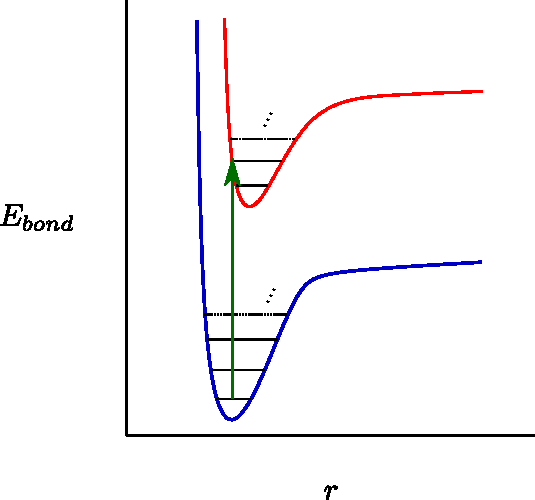
\includegraphics[width=0.5\linewidth]{../figures/potential_energy_curve.pdf}
    \end{center}
    \caption{A visualization of vibronic transitions. The blue and red curves represent H$_2$ and H$_2^+$, respectively.}
        \label{fig:visualize_vibronic}
\end{figure}

You are provided with a \texttt{python} notebook called \texttt{Task1.ipynb} which calculates all of the information you require. The \texttt{FCF\_helper.py} file contains all of the calculations done under the hood. \footnote{Calculating FCFs comes down to calculating the overlap between the wavefunctions before and after the vibronic transition. The overlap calculation is an integral which we chose to evaluate numerically. We emphasize that molecular parameters like the reduced mass of H$_2$ and fundamental frequencies of H$_2$ and H$_2^+$ are hard-coded in \texttt{FCF\_helper.py}} Currently, the \texttt{spectrum\_analysis} function in \texttt{FCF\_helper.py} only outputs the following.
\begin{itemize}
    \item \texttt{n\_0} and \texttt{n\_p}: The vibrational state numbers of H$_2$ and H$_2^+$, respectively, involved in the vibronic transition
    \item \texttt{FCF}: The corresponding FCF associated to the vibronic transition
\end{itemize}
Here's what we'd like you to do:
\begin{enumerate}
    \item Open up \texttt{FCF\_helper.py} and navigate to the \texttt{spectrum\_analysis} function. Modify the \texttt{data} variable so that it also includes the spectral intensity (\texttt{Ep - E0}).
    \item Plot the corresponding FCF versus spectral intensity (i.e. plot \texttt{FCF} versus \texttt{Ep - E0}) and show the results for \texttt{n\_0}=0 and \texttt{n\_p}=10.
\end{enumerate}

Congratulations, you have now successfully predicted the Franck-Condon Factors of H$_2-$H$_2^+$! Figure \ref{fig:h2_spectrum} shows the photoionization spectrum for H$_2$. Does it look like the real data in Fig.~\ref{fig:h2_spectrum}?

\begin{figure}
    \begin{center}
        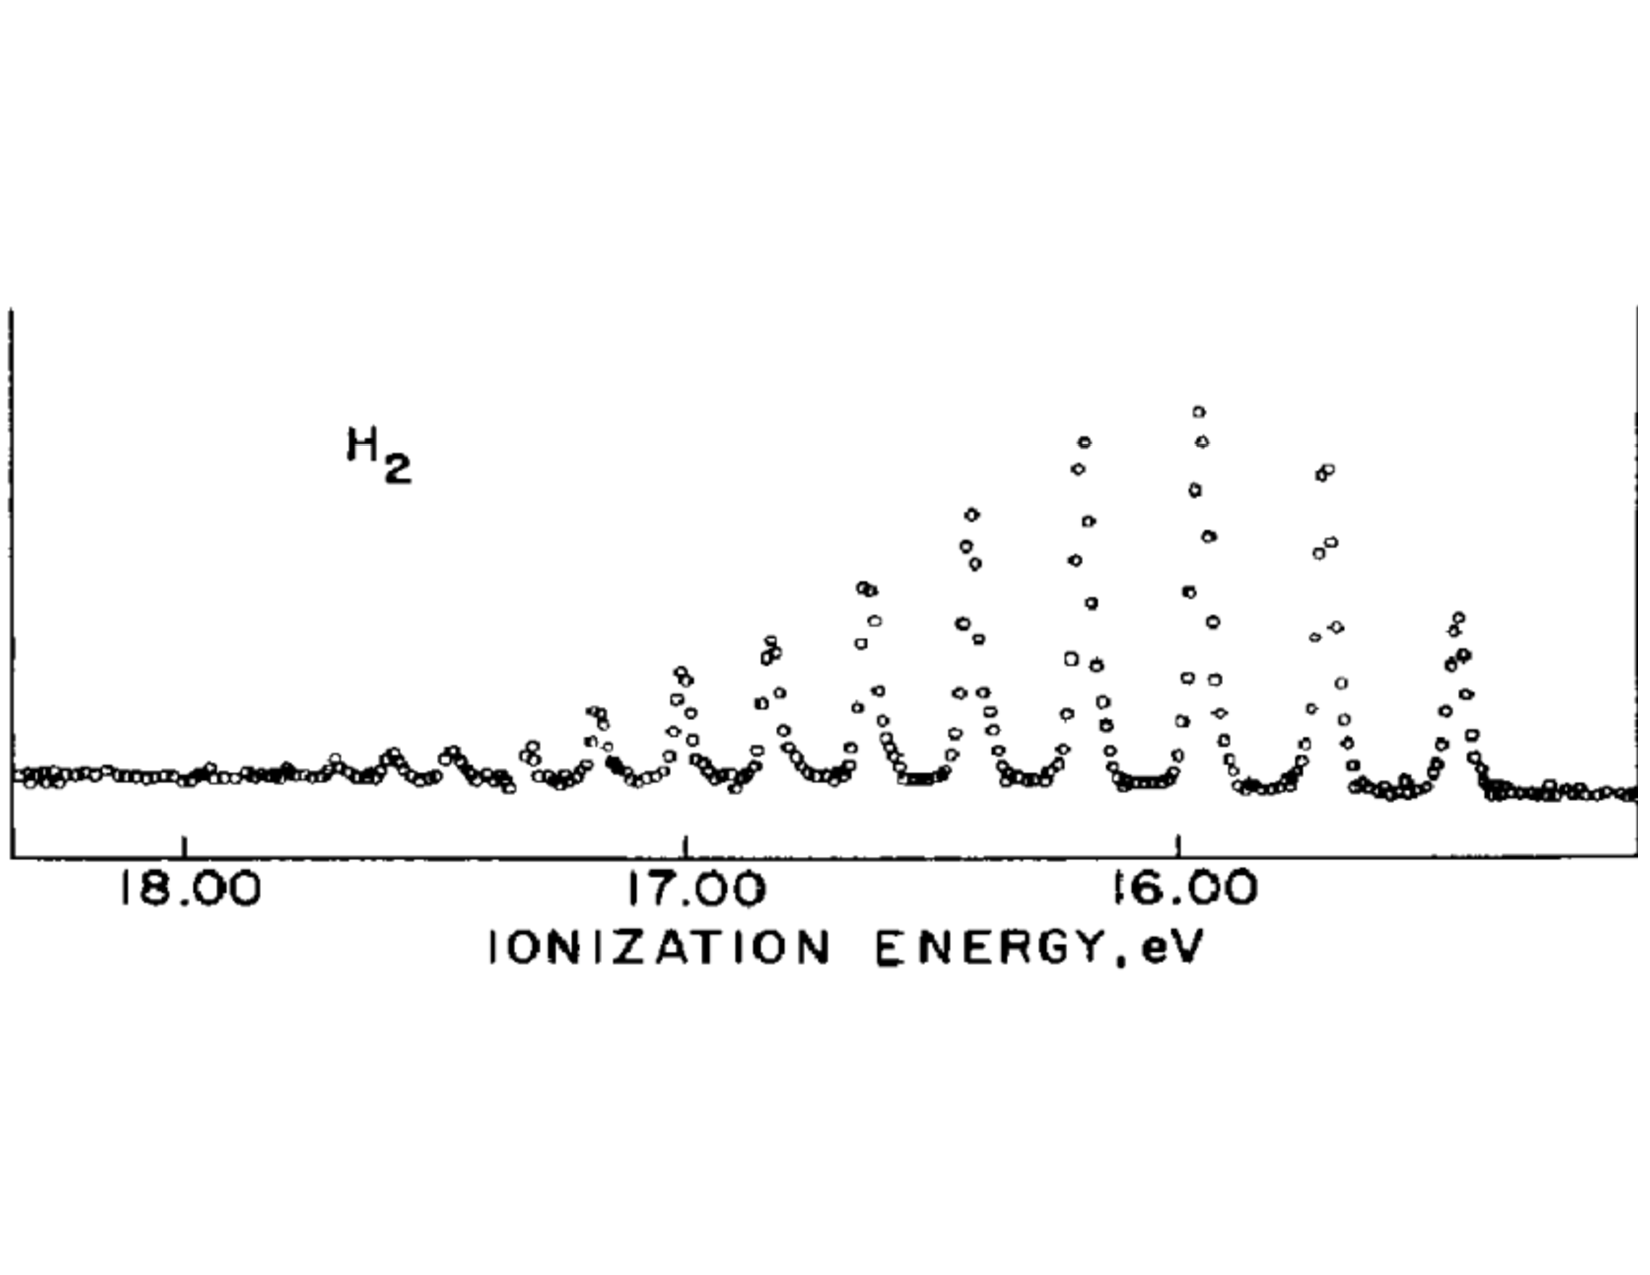
\includegraphics[width=\linewidth]{../figures/H2-expspectrum.pdf}
    \end{center}
    \caption{
    Experimental photoionization spectrum of H$_2$-H$_2^+$ from Ref.~\cite{berkowitz1973comparison} with the vibrational level of H$_2$=0.
    }
    \label{fig:h2_spectrum}
\end{figure}

\subsubsection*{Task \#2}

You are provided with a \texttt{C++} code \texttt{FC.cxx} created by P.-N. Roy \cite{yang1995structure}, which calculates the photoionization spectrum for any molecule up to triple excitations and goes beyond the harmonic oscillator approximation. The theory is based on the paper by Ref~\cite{doktorov1977dynamical}. The molecule you will be investigating is $V_3$.
This code takes as input a file which requires the results of diagonalizing the mass-weighted hessian/force-constant matrix (2nd derivative of the Hamiltonian with respect to position). This input file is provided for you (V3).

Browse the following references (\cite{yang1995structure,doktorov1977dynamical,quesadaFranckCondonFactorsCounting2019}) to understand how the code works, as you will need a basic understanding of this for the next task, but it's not necessary to fully understand it.  Compile and run the code \texttt{./FC\_quick V3}. This code outputs the spectrum \texttt{V3.spec.out}. Plot it in your favourite plotting program. 

\subsubsection*{Task \#3}

In this task, you will be simulating a Gaussian Boson Sampling (GBS) ``experiment." This code generates samples for computing a vibronic spectrum. Each sample that is generated starts from the vacuum state and the following gates are performed\cite{killoran2019strawberry, bromley2020applications}.

\noindent This code takes as input a file which requires the following information:
\begin{enumerate}
\item Two-mode squeezing on all  $2N$  modes with parameters \texttt{t}
\item Interferometer \texttt{U1} on the first $ N$ modes
\item Squeezing on the first $N$ modes with parameters \texttt{r}
\item Interferometer \texttt{U2} on the first  $N$ modes
\item Displacement on the first  $N$ modes with parameters \texttt{alpha}
\end{enumerate}

The energy of the resultant state is calculated and contributes to the spectrum. After running this simulation over many samples and plotting the energies against their frequency, those states (energies) with a high Franck-Condon Factor will have a larger peak on the spectrum and those with a low Franck-Condon Factor will have a smaller peak. It is important to note that it's not the exact values of the peak heights that we care about in this case (since it's based on a probability distribution), it's the relative heights of the peaks of the spectrum.

\hspace{20mm}

You are provided with a \texttt{python} notebook called \texttt{Task3.ipynb} which calculates all of the information you require. You will be required to use the \texttt{Strawberry Fields} library\cite{killoran2019strawberry, bromley2020applications}. Click  \href{https://strawberryfields.readthedocs.io/en/stable/_static/install.html}{\underline{\textbf{here}}} for the install instructions. However, to be able to use this code, you require an input file, which you will have to create. To do this, we will leverage the fact that we have another code that has done this work already, \texttt{FC.cxx}, which you became familiar with in Task 2. Each piece of information that you need to output has been clearly marked in the code and your task is to write that information to a file, which will then be used as your input file to \texttt{Sample\_Vibronic.py}. Once you have that input file, you should be able to produce the spectrum for $V_3$. Compare this spectrum to the previous method. What happens if you decrease the number of samples to 10? 100? 1000? At what number of samples do you feel the spectrum is converged?

\section*{Challenges}

\begin{enumerate}
    \item An alternative and analogous method to calculating these Franck-Condon Factors using matrix elements is to use a loop hafnian approach. This loop hafnian approach uses Gauss Boson Sampling which would allow these Factors to be calculated using a quantum circuit. Use the result of Task 3 to provide data to a skeleton code provided that uses loop hafnians to calculate the Franck-Condon Factors.
    \item Explain briefly the similarities and differences between these three methods.
\end{enumerate}

\section*{Possible Business Outcomes}

\begin{enumerate}
    \item Explain to a layperson what theoretical chemistry/physics is, in the general context of Franck-Condon Factors.
    \item What is the importance of theoretical chemistry/physics from an economic point of view.
    \item Explain to a layperson what a quantum circuit is and its relationship to theoretical chemistry/physics.
    \item These codes use General Public License and Apache 2.0 licenses. Discuss the similarities and differences of these with respect to intellectual property rights of the coder. What are the advantages and disadvantages of codes licensed for the public domain and those that are licensed for private use.
\end{enumerate}

\newpage

\bibliography{refs}
\bibliographystyle{unsrt}

\end{document}
